\documentclass[sigconf,nonacm,11pt]{acmart}

\begin{document}
\title{Chevrotain: A Conflict-free Replicated Data Type Key-Value Store}

\author{Alexandre Avreline}
\email{savrelin@students.cs.ubc.ca}
\affiliation{%
  \institution{Univeristy of British Columbia}
  \city{Vancouver}
  \state{British Columbia}
  \country{Canada}
} 

\begin{abstract}
Chevrotain is a replicated key value store that achieves eventual consistency through the use of a conflict-free replicated data types (CRDTs). This paper describes the designs, evaluates performances, and compares three different approaches to the implementation of Chevrotain. One of the approaches is based on a state-based CRDT model (CvRDT), while the other two approaches are based on an operation-based CRDT model (CmRDT), that is either completely unsynchronized or makes limited use of synchronization. Latency of all implementations is measured as a function of throughput, and consistency of all implementations is compared to a simple replicated key-value store that only makes a minimal effort to maintain consistency. Scalability of all implementations is also studied. Results shows that the unsynchronized CmRDT implementation of Chevrotain demonstrates the best performance. In particular, this implementation easily scales to ten geographically distant replicas, achieves sub-second latency under a throughput of 100 ops/second while maintaining perfect eventual consistency. A proof-of-concept application to distributed web crawling is also presented.\end{abstract}

\keywords{eventual consistency, conflict-free replicated data types, key-value stores}

\maketitle

\section{Introduction} 
% Testing citation \cite{Davey:Lattices}
% Testing referencing \ref{fig:sys}

In distributed systems there is always the tension between maintaining consistency and demonstrating high performance. On one end of the spectrum there is strong consistency which implies that the distributed system behaves like a single machine that serializes all operations. Strong consistency maintains perfect data consistency at all times, at the expense of high latency due to the need for synchronization and constant communication between nodes. On the other end of the spectrum is eventual consistency which allows for the states of the distributed replicas to temporarily diverge and meet later in time. Eventual consistency results in a lower frequency of communication which leads to better performance; however, eventual consistency could lead to data inconsistencies and data loss \cite{li2012making}. 

Some of the recent research focused on trying to strike a balance between strong consistency and high performance. This has led to the emergence of mixed consistency semantics, such as RedBlue consistency, consistency rationing, PSI and Horus \cite{li2012making},\cite{kraska2009consistency},\cite{sovran2011transactional},\cite{van1996horus}.  In such semantics, strong consistency is enforced on the operations that depend on the data to be immediately consistent, while weak consistency is used with operations for which a high degree of consistency is not necessary. An alternate approach is for programmers to design the distributed system in a way that does not require strong consistency at all. This is the approach that is used in concept of conflict-free replicated data types (CRDT) \cite{shapiro2011conflict}, which is the focus of this paper.

In CRDTs, the distributed system is designed such that either the states of replicas could be merged in a conflict-free way at any point in time (state-based RDT or CvRDT) or that any updates to the states of the replicas are only done in a conflict-free way (operation-based RDT or CmRDT) \cite{shapiro2011conflict}. This paper presents the design, implementation and performance evaluation of Chevrotain, a CRDT-based key-value store. Three different approaches to implementation of Chevrotain are considered. One of the approaches is based on the CvRDT model, while the other two approaches are based on the CmRDT model, either with or without limited synchronization.

Key-value stores present a flexible data storage model that has widespread use, which allows Chevrotain to be appropriate tool for a variety of applications. We present one such application, a distributed web crawler, in section 5.

This paper begins by briefly describing the mathematical foundations behind CRDTs in section 2. The designs of all proposed implementations of Chevrotain are then detailed in section 3. Section 4 presents the performance evaluation results, while sections 5-8 briefly survey applications, future work, related work and present the conclusion.
 
\section{Background}
\subsection{CvRDT}
In state-based replication, each update that is executed at a replica modifies the state of that replica. Then, at specified intervals in time, every replica broadcasts its local state to the other replicas, which merge the received state into its own \cite{shapiro2011conflict}.

For the merges to be conflict-free, the states of replicas must resemble a monotonic semilattice object. A monotonic semilattice is a term from mathematical set theory \cite{Davey:Lattices} but in the context of CRDTs it means the following \cite{shapiro2011conflict}:
\begin{itemize}
 \item there is a partial order that could be used to order the states,
 \item the merge operation computes the least upper bound (defined below) of the two states, and
 \item the states are monotonically non-decreasing across updates (as in the state that follows an update is ordered after the state that precedes the update).
\end{itemize}

As mentioned, the merge operation must compute the least upper bound of the local and incoming states. The least upper bound (or join) is another term from set theory \cite{Davey:Lattices} that effectively means that the merge operation determines the maximal state of the local and incoming states.

The original work on CRDTs \cite{shapiro2011conflict} provides some examples of what determining maximal state during the merge might look like. The classical example is vector clocks where the merge method takes the maximum of each respective entry. Another classical example provided by \cite{shapiro2011conflict} is concerned with merging logs: the merge method just takes the union of the local and incoming logs.

A key-value store could be represented by a collection of sets that consists of a set of keys and a set of values for each key. There are several state-based CRDT frameworks for sets and one such framework is the LWW-element-set (last-write-wins-element-set). In this framework, for any set, two sets are maintained: an ``add'' set and a ``remove'' set. Elements are added to the LWW-element-set by being added to the add set and are removed from the LWW-element-set by being added to the remove set. All additions and removals are marked with Lamport timestamps. An element is a member of the LWW-element-set if it is a member of the add set and is either not in the remove set or is in the remove set but is marked with an earlier timestamp than is marked in the add set. In the case when the timestamps of the element in the add and remove sets are identical, a user-defined bias towards either the add or the remove operations comes into play. Merging two replicas of an LWW-element-set entails taking the union of the respective add and remove sets \cite{shapiro2011comprehensive}.

\subsection{CmRDT}
The other approach to CRDTs is operation-based. Instead of having replicas periodically exchange states, whenever an update is executed at some replica, that update is propagated to other replicas using a casual broadcasting communication protocol (CBCAST) \cite{baldoni2002fundamentals}. Then there are two possible scenarios:
\begin{itemize}
 \item either the updates are ordered by CBCAST and are executed in that order at each replica, or
 \item the updates appear to be concurrent.
\end{itemize}

In the first scenario there are no issues and no conflicts. However, if the updates appear to be concurrent, then one of the following must be the case:
\begin{enumerate}
 \item either the updates are commutative (as in, the order in which they are applied at a replica is irrelevant and either order results in the same final state), or
 \item the updates are delayed until all concurrent updates have been received and any conflicts between those updates are resolved in a systematic way, or
 \item some other, application-specific approach is formulated that allows concurrent updates to proceed without any synchronization.
\end{enumerate}

It is not the case by any means that all operations are commutative; therefore, some of the updates will require resorting to approaches described by either 2 or 3 above. In this paper, we will present a conservative implementation approach that follows the approach of point 2 and requires a limited degree of synchronization between replicas. This approach will be referred to as CmRDT-C. We will also present a more optimistic implementation approach, that follows the approach of point 3 and requires no synchronization. This approach will be referred to as CmRDT-O.

\section{Design and Implementation}
The general system layout, that is the same across all implementations, is shown in figure \ref{fig:sys}. The entire implementation is written in Golang and each replica contains a local copy of a MongoDB 4.4 database. A client communicates with replicas by making RPC calls to the methods made available by the RPCExt object. The methods available to a client through the RPCExt object are the following:
\begin{itemize}
 \item InitReplica (timeInt int, bias Bias)
 \item InsertKey (key string)
 \item InsertValue (key string, value string)
 \item RemoveKey (key string)
 \item RemoveValue (key string, value string)
 \item TerminateReplica ()
\end{itemize}

The InitReplica method initializes the replica's internal data structures and establishes its connections to other replicas. A group membership file that lists other replicas' IP addresses and port numbers is provided for this purpose. Once a replica has been initialized, a client sends commands to the replica by the virtue of the remaining methods. In the CvRDT implementation, commands are processed locally, and state updates are broadcast to other replicas periodically with a time interval specified by the timeInt argument. In the CmRDT implementations, commands are processed locally and are then immediately broadcast to other replicas. All inter-replica communication happens through the methods made available by the RPCInt object, the exact make up of this object is implementation specific.

\begin{figure}[h]
  \centering
  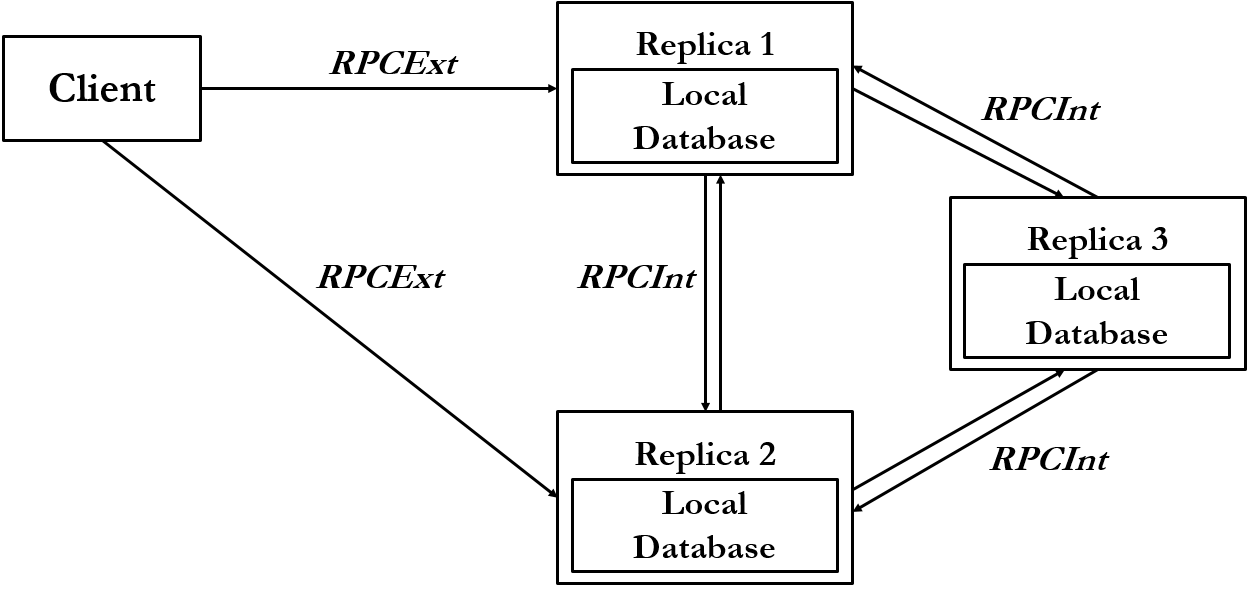
\includegraphics[width=\linewidth]{Fig1Sys}
  \caption{General System Layout}
  \label{fig:sys}
\end{figure}

\subsection{CvRDT}
A typical workflow of the CvRDT implementation is shown in figure \ref{fig:cvrdt1}. Each local copy of the database holds two collections: a positive collection and a negative collection. The collections respectively store all the ``add'' and all the ``remove'' sets of the LWW-element-set. We will refer to positive and negative collections as the dynamic collections. 

\begin{figure*}[h]
  \centering
  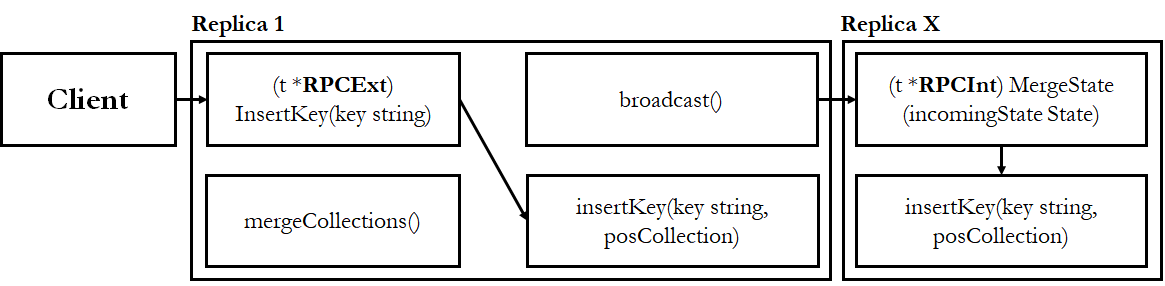
\includegraphics[width=15cm]{Fig2CvRDT1}
  \caption{Typical CvRDT Workflow}
  \label{fig:cvrdt1}
\end{figure*}

Suppose a client makes an RPCExt call to the InsertKey method. Since a key is being inserted, this key will be immediately added to set of all keys in the positive collection (had the RemoveKey method been called, the key would been added to the same set in the negative collection) along with the current Lamport clock timestamp. Then, at predetermined time intervals, specified at replica's initialization, the entire state of the local database will be downloaded and broadcast to all other replicas. This is done by calling the MergeState method of the RPCInt object on each replica. Once a replica receives the incoming state, it merges that state with its own state, by taking the union of the corresponding sets in the corresponding collections. In particular, during this merge, a replica adds any missing elements to the correct set in its database. When merging dynamic collections, elements are considered identical if and only if their values and timestamps are identical.

The mergeCollections method merges the positive and negative collections into a single collection, referred to as the static collection. This method compares the timestamps of all instances of a given element across both collections. It then inserts the element into the static collection if and only if its largest timestamp in the positive collection is greater than its largest timestamp in the negative collection. Should the element's largest timestamps in the positive and negative collections be the same, the element is inserted into the static collection if indicated so by the bias set at replica's initialization. The bias tends to be application specific and is left to be specified by the end-user.

In a basic implementation, the mergeCollections method needs to run only whenever the user wishes to access the data. However, such an approach leads to replicas always broadcasting the entire states of their local databases and substantially degrades performance. Therefore, in Chevrotain, the mergeCollections method runs following each state broadcast. This approach, which is also known as garbage collection, adds complexity but improves performance. Replicas agree on a \emph{current safe tick} of the Lamport clock and all entries of the positive and negative collections that are timestamped with timestamps smaller than this tick are moved into the static collection. Those elements are also removed from the positive and negative collections at the same time, significantly reducing the size of the state that needs to be broadcast.

Figure \ref{fig:cvrdt2} shows an example of how mergeCollections works in practice. Suppose the current safe tick is 8; therefore, element 3 will be inserted into the static collection as just the entry \{``3'', 6\} of the positive collection for element 3 is considered at this time. Should there be no further entries for element 3, it will be removed from the static collection on the next iteration once the entry \{``3'', 10\} is processed. Likewise, element 4 will not appear in the static collection at this time as the entry \{``4'', 5\} of the negative collection dominates over the entry \{``4'', 2\} of the positive collection and the entry \{``4'', 9\} has not been processed yet.

\begin{figure}[h]
  \centering
  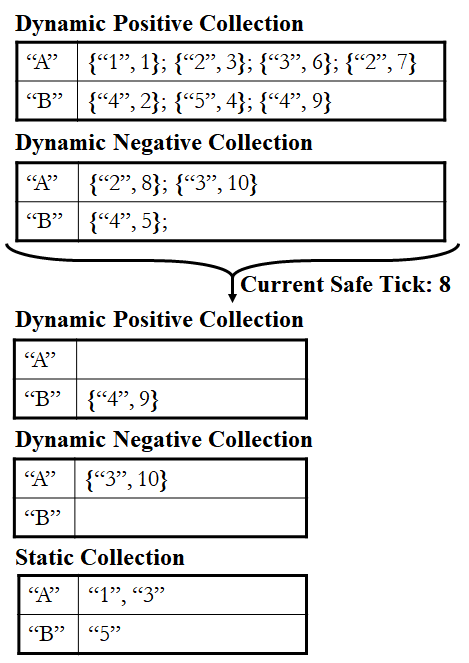
\includegraphics[width=6.25cm]{Fig3CvRDT2}
  \caption{Management of LWW-Element-Sets in CvRDT}
  \label{fig:cvrdt2}
\end{figure}

In the current rather simple implementation, for all replicas to agree on the current safe tick, a replica designated as a leader collects the current timestamp ticks from all replicas as replies to state broadcasts. It then takes the minimum among those ticks and of its own current tick. The resulting tick is included in the following state broadcast. Other replicas then accept the leader mandated current tick. A more robust implementation is considered in section 6 future work.

Replicas wait for the incoming state broadcast to be merged into the local state prior to merging the collections together. This, along with the agreement on the current safe tick, ensures that elements are moved in exactly same blocks into the static collection at all replicas when merging. This level of determinism ensures there is no loss of consistency due to merges and elements with equivalent timestamps are processed in the same way at all replicas.

\subsection{Types of Conflicts in CmRDT}
Prior to going into the details of the CmRDT implementations, we will investigate the types of conflicts that can arise between concurrent operations in the context of a key-value store. The specific conflict resolution mechanisms will be implementation specific. The operations that operate on different keys or on different key-value pairs are commutative and can proceed in any order. As far as the other operations are concerned, the following two types of conflicts can arise.

We will refer to the conflicts that arise between the following pairs of concurrent operations operating on the same key or on the same key-value pair as type I conflicts:
\begin{itemize}
 \item InsertKey, InsertValue
 \item RemoveKey, RemoveValue
\end{itemize}

Likewise, we will refer to the conflicts that arise between the following pairs of concurrent operations operating on the same key or same key-value pair as type II conflicts:
\begin{itemize}
 \item InsertKey, RemoveKey
 \item InsertValue, RemoveValue
\end{itemize}

\subsection{CmRDT-O: Optimistic Approach}
The implementation of CmRDT-O is largely an adoption of the implementation of a graph CRDT that is described in section 5 of \cite{shapiro2011conflict} to a key-value store. Each operation is split into prepare-update and effect-update methods. The prepare-update method is side-effect free and takes place only at the replica to which the operation was initially delivered to. The effect-update method applies the operation to the local database and runs at each replica.

A typical workflow of the CmRDT-O implementation is shown in figure \ref{fig:cmrdtb}. The CmRDT-O database initially maintains a collection of a set of keys and sets of values for each key. This collection will be referred to as the dynamic collection. In this collection, each instance of each element is tagged with a unique id. When inserting a key or a value, the prepare-update method generates a unique id for the key or the value. The element-id pair is then immediately inserted into the local database by the effect-update method and is also broadcast to all other replicas to be processed by the effect-update methods there (in particular, the element will be inserted into the databases with the same id at all replicas). A lock is used to ensure that the effect-update method immediately follows the prepare-update method at the initiating replica.

\begin{figure*}[h]
  \centering
  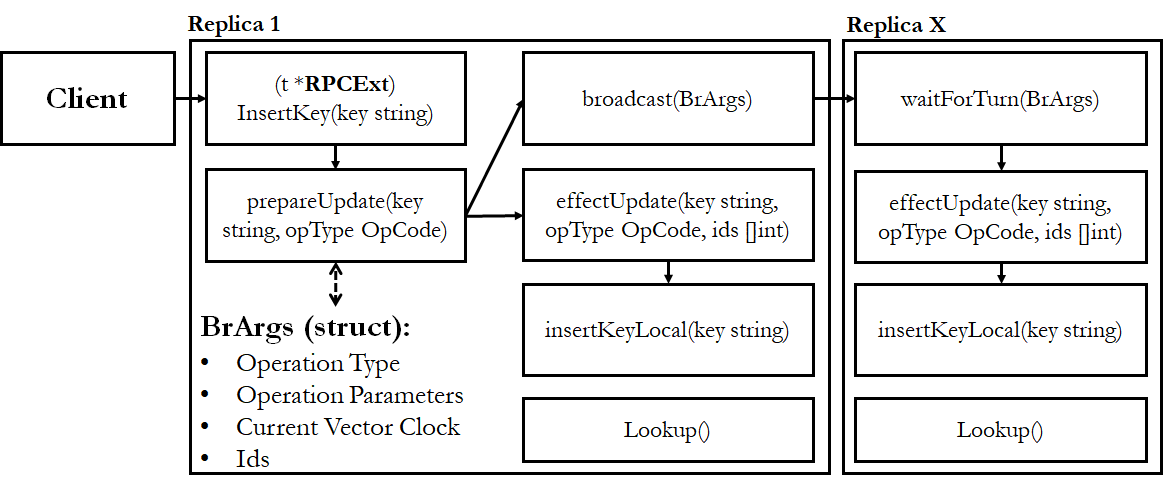
\includegraphics[width=15.5cm]{Fig4CmRDTB}
  \caption{Typical CmRDT-O (Optimistic Approach) Workflow}
  \label{fig:cmrdtb}
\end{figure*}

When removing a key or a value, the prepare-update method generates the ``removal'' set which contains the unique ids of all instances of the given element. The effect-update then removes all those instances from the local database. Finally, the element-ids pair is broadcast to all other replicas for removal by the effect-update methods there (in particular, all replicas will remove the exact same instances of the given element).
Broadcasts are to be ordered according to the vector clocks and therefore the incoming broadcasts are held at each replica until the correct broadcast arrives. To achieve this, a channel is established to communicate with each incoming RPCInt call. The channel of any RPCInt call that is waiting on new broadcast messages to arrive is added to a dynamic pool. Whenever the correct broadcast message arrives, the updated local vector clock is broadcast to the channel pool to see if any of the waiting RPCInt calls can proceed next. The GoVector package was adapted to provide the vector clock functionality required for casual broadcasting \cite{distributedclocks}.

Fixation of the removal set by the prepare-update method addresses the type II conflicts. There cannot be a concurrent InsertKey and RemoveKey coming from the same replica as those would be ordered by vector clocks on that replica. Should there be a concurrent InsertKey and RemoveKey coming from different replicas, InsertKey will take precedence as the removal set associated with the call to RemoveKey will not include the just-generated unique id of the instance of the element to be inserted.

Type I conflicts are resolved by allowing an InsertValue to proceed to the local database even if the corresponding InsertKey has not arrived yet. Whenever an end-user wishes to start looking up keys or values in the database, the dynamic collection is transformed into what is referred to as the static collection by the lookup method. This method presents a simple view of the data without the unique ids and it also hides any inconsistencies. In particular, should the InsertKey method never arrive, the inserted value will not be copied over to the static collection and will not be displayed whenever a user looks it up in the database. RemoveKey and RemoveValue conflict is addressed in a similar way.

\subsection{CmRDT-C: Conservative Approach}
In the CmRDT-C implementation, a queue is used to order operations at each replica and to resolve any conflicts that arise between concurrent operations in a pre-determined, systematic way. A typical workflow of the CmRDT-C implementation is shown in figure \ref{fig:cmrdtq1}. When a replica receives a command from the client, it immediately timestamps the command with the current vector clock and packages the command into an OpNode struct. The OpNode struct, along with the timestamp, contains all necessary information to process the command. The OpNode struct is then inserted into the local queue of OpNodes, where the OpNodes are ordered according to vector clocks. Finally, the OpNode struct is also broadcast to all other replicas, where upon arrival, it is likewise inserted into the local OpNodes queues. The queue insertion mechanism first tries to locate an OpNode whose timestamp is either ahead or behind the timestamp of the incoming OpNode. If such an OpNode does not exist, then the incoming OpNode is placed next to an OpNode with a concurrent timestamp. Therefore, the queue may have one or more blocks of one of more concurrent operations, as is shown in figure \ref{fig:cmrdtq2}.

\begin{figure*}[h]
  \centering
  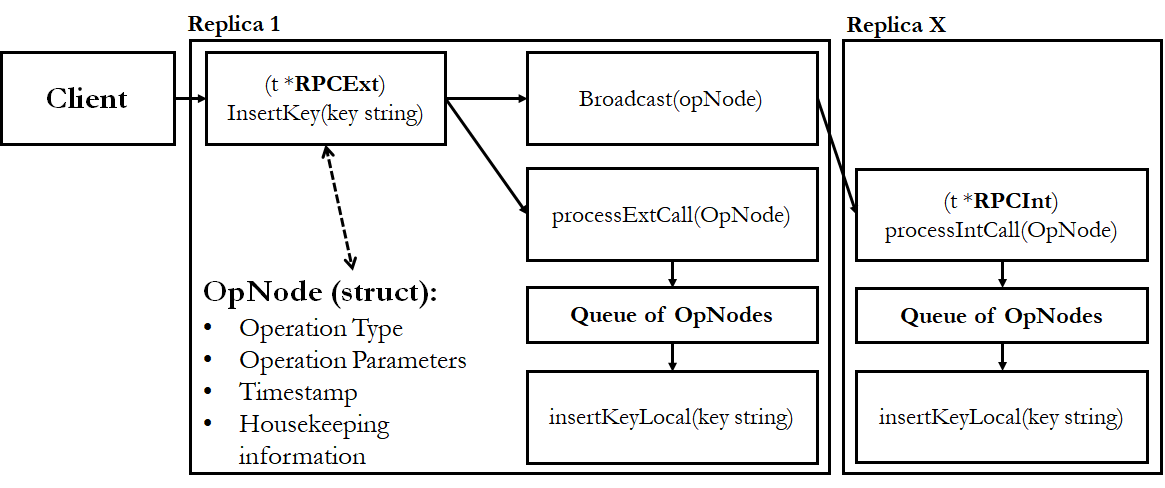
\includegraphics[width=15.5cm]{Fig5CmRDTQ1}
  \caption{Typical CmRDT-C (Conservative Approach) Workflow}
  \label{fig:cmrdtq1}
\end{figure*}

\begin{figure*}[h]
  \centering
  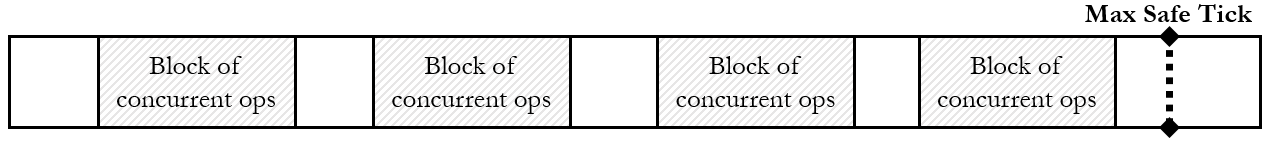
\includegraphics[width=15.5cm]{Fig6CmRDTQ2}
  \caption{Queue of Operational Nodes in the CmRDT-C}
  \label{fig:cmrdtq2}
\end{figure*}

Whenever the queue of OpNodes reaches a certain predetermined length or a certain amount of time has passed, it is processed to resolve any conflicts between any concurrent operations. The processed operations are removed from the queue and are applied to the local database. Only the OpNode whose timestamps can no longer be concurrent to the timestamps of any forthcoming OpNodes are processed. To determine this point on the queue, a \emph{maximum safe tick} is computed by taking the minimum of the maximum clock ticks seen from all replicas. 

For example, suppose that some replica has seen the OpNodes with the following vector clocks. Then the maximum clock tick seen from replica 1 is 3, is also 3 from replica 2 but is only 2 from replica 3. Therefore, the maximum safe tick in this case is $\min\{3,3,2\}$ which is 2. Therefore, only the first six OpNodes will be processed as this point in time, as all entries of the timestamps of those OpNodes are less than or equal to the current maximum safe tick. In particular, it might still be possible to receive an operation whose timestamp is concurrent to the timestamp of the seventh OpNode, such a timestamp would be [2,2,3] coming from the third replica. However, it is no longer possible to receive an operation whose timestamp would be concurrent to any of the first six timestamps.

$$ \underbrace{\begin{bmatrix} 1\\0\\0 \end{bmatrix},
\begin{bmatrix} 0\\1\\0 \end{bmatrix},
\begin{bmatrix} 0\\1\\1 \end{bmatrix},
\begin{bmatrix} 1\\2\\1 \end{bmatrix},
\begin{bmatrix} 2\\2\\1 \end{bmatrix},
\begin{bmatrix} 2\\2\\2 \end{bmatrix}}_{\text{only those are processed at this time}}, 
\begin{bmatrix} 3\\2\\2 \end{bmatrix},
\begin{bmatrix} 3\\3\\2 \end{bmatrix}$$

In order to ensure that clock ticks of different replicas do not grow far apart and hold up processing, replicas that do not have any operations to contribute will send no-ops at time intervals specified by the timeInt argument to the InitReplica RPCExt call.

Once the queue has been cut off at the maximum safe tick for processing, any conflicts found in the blocks of concurrent operations are addressed. First, blocks of concurrent operations are scanned to determine if there are any conflicts to be addressed. For a given block of concurrent operations, there are two cases in which we can safely say there would not be any conflicts:
\begin{itemize}
 \item all operations within the block operate on different keys and values, or
 \item all operations within the block are of the same type (for example, all operations are InsertKey)
\end{itemize}

If a block of concurrent operations falls into either of the above categories, it is left as is. Otherwise, operations within the block are reordered to address any type I or type II conflicts. With respect to type I conflicts between concurrent InsertKey and InsertValue operations that operate on the same key, InsertKey is ordered to proceed first. Likewise, between concurrent RemoveKey and RemoveValue operations that operate on the same key-value pair, the RemoveValue is ordered to proceed first. As for type II conflicts, they are resolved in the same way as in the CvRDT implementation: as per the user specified bias. As in the CvRDT implementation, the bias towards adds or removes is passed as an argument to the InitReplica RPCExt call.

\section{Evaluation}
\subsection{Methodology}
The basic evaluation of throughput, latency and consistency of all implementations was carried out using three Microsoft Azure Standard DS1 VMs running Windows 2019 Datacenter Server with 1 vCPUs, 4GB of RAM and a separate premium SSD drive dedicated to Chevrotain. The initial VMs were geographically distributed and situated in Central Canada, Southern UK and Japan East.

A standard test set suite was used to collect all measurements: at the beginning of the test, 50 key insertion commands were sent to each replica, immediately followed by 20 value insertion commands on each key. In the middle of the test, some additional keys and key-value pairs were repeatedly inserted and removed. Finally, at the end of test, half of the values from each key and one-fourth of the keys were removed. The beginning and end portions of the test were meant to introduce type I conflicts, while the middle portion was meant to introduce type II conflicts. In all experiments, each test was done three times and reported results are the average of the three runs.

The client sent all commands asynchronously and was responsible for recording round trip latencies of each RPCExt call. The client introduced set delays between subsequent sends to emulate various levels of throughput. A ``zero'' implementation was used as a baseline reference. This implementation still followed the system layout outlined in figure \ref{fig:sys}; however, once operations were received by the replicas, they were immediately applied to the local databases, without any additional processing to improve consistency.

A checker package was also put together. This package connects to the local copies of the databases at each replica and cross-checks them for consistency. The consistency results are reported as a percentage of entries that match across the databases. 

\subsection{Throughput and Latency Results}
Measurements of latency as a function of throughput for different implementations are presented in figure \ref{fig:eval1}.

\begin{figure}[h]
  \centering
  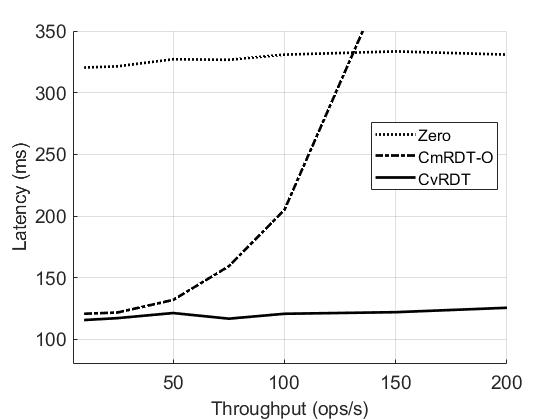
\includegraphics[width=\linewidth]{Fig7Eval1}
  \caption{Latency as a Function of Throughput}
  \label{fig:eval1}
\end{figure}

\subsection{Consistency Results}
Measurements of consistency as a function of throughput are presented in figure \ref{fig:eval2}. 

A particular problem with achieving consistency in the CmRDT-C implementation is the maximum length of the queue. Ordering of OpNodes in the queue according to vector clocks is not unique and as the queue grows in size, this non-uniqueness becomes more problematic.

\begin{figure}[h]
  \centering
  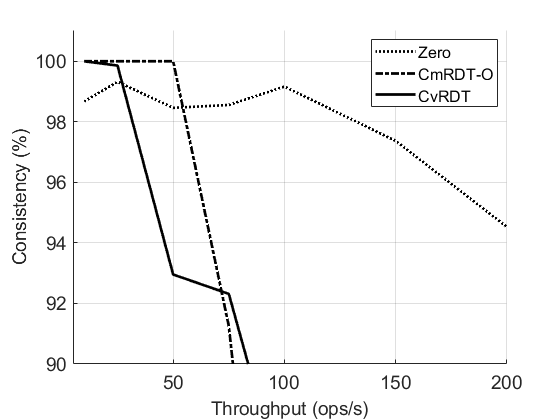
\includegraphics[width=\linewidth]{Fig8Eval2}
  \caption{Consistency as a Function of Throughput}
  \label{fig:eval2}
\end{figure}

\subsection{Scalability Results}
To measure scalability of each implementation, additional identical Microsoft Azure VMs were added in the following regions: Australia, Brazil South, US West and Africa. Results are presented in figure \ref{fig:eval3}.

\begin{figure}[h]
  \centering
  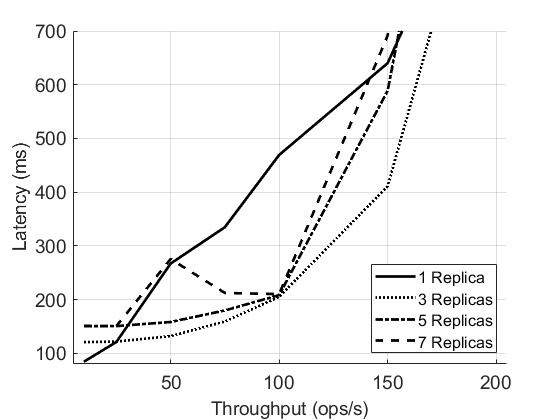
\includegraphics[width=\linewidth]{Fig9Eval3}
  \caption{Scalability of the CmRDT-O Implementation}
  \label{fig:eval3}
\end{figure}

\section{Applications and Use Cases}
There are numerous applications of replicated key-value stores. Some of the simpler ones include basic hash tables that could be used to store usernames and passwords or a list of network servers and their current statuses. One slightly more involved application is a distributed web crawler that builds a web page link directed graph (DG). Starting from some page on the web, a DG could be constructed to capture the relationship between web pages reachable from that page. Each page is represented by a vertex and each link is represented by an edge. Such DGs are used in the Page Rank algorithm originally invented by Google \cite{brin1998anatomy}.

Any graph could be represented as a key-value store with the keys being vertices and values for each key capturing the list of neighboring vertices to that the vertex. See figures \ref{fig:wiki1} and \ref{fig:wiki2} for an example of web page link DG and its representation as a key-value store.

\begin{figure}[h]
  \centering
  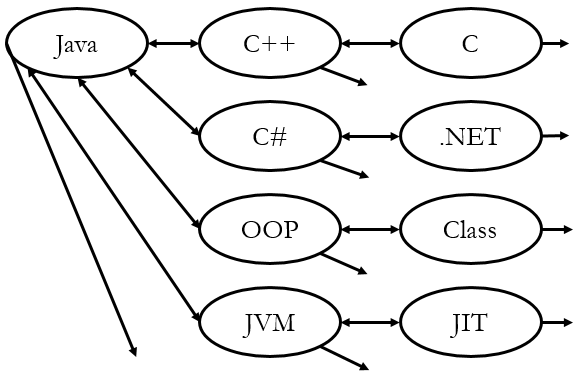
\includegraphics[width=7cm]{Fig11Wiki1}
  \caption{Sample Web Page Link Directed Graph}
  \label{fig:wiki1}
\end{figure}

\begin{figure}[h]
  \centering
  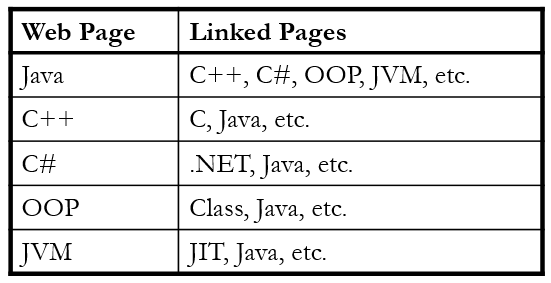
\includegraphics[width=7cm]{Fig12Wiki2}
  \caption{Adjacency List Representation of a Sample Web Page Link Directed Graph}
  \label{fig:wiki2}
\end{figure}

The web page link DG framework was built a as an application proof-of-concept to Chevrotain. A client communicating with a certain replica is given a starting Wikipedia page (for example ``Java'') and crawls any webpages originating from that page up to a certain depth, sending commands to Chevrotain to insert keys and values as pages are traversed. Other clients are given other starting webpages and send commands to their respective Chevrotain replicas. Chevrotain replicas then replicate the commands or exchange state to arrive at a uniform view of the Wikipedia page DG. The Chevrotain implementations were tested using this framework and achieved perfect eventual consistency; however, this framework was not used for any benchmark measurements at this time.

\section{Future Work}
Future work on this project would involve making Chevrotain more robust to failures and more optimized for performance. One of the goals would be to equip the CvRDT implementation with a better protocol for reaching agreement on the current safe tick among all replicas and responding to leader failures. In particular, Golang Paxos implementations \cite{paxos} could be explored to address this. Another goal would be to have CmRDT implementations be better suited to handle lengthy replica failures: should a replica be offline for an extended period of time, it would receive the entire state update as a single message, rather than receiving a series of messages containing individual operations.

Other test suites should be explored to gather performance measurements and evaluate robustness of Chevrotain. In particular, it would be interesting to discover test suites that perform very well with some implementation of Chevrotain and poorly with others.

A more interesting web crawling experiment would be to have Chevrotain replicas situated in different geographical regions crawl web pages located in those regions and only occasionally exchange states between themselves. In particular, it would be interesting to see if there would be a performance gain in comparison to a web crawler situated in a single region crawling pages from all over the globe from there.

\section{Related Work} %MongoDB!!!
The use of CRDTs is very widespread and there are several excellent CRDT libraries, most of them are written in JavaScript \cite{crdt}. Many of those are domain specific and not directly related to key-value stores, such as the \textbf{Automerge} library for JSON files \cite{automerge}. However, many modern databases either support or are adapted to support CRDT frameworks. One example is the \textbf{Microsoft Azure CosmosDB} that supports CRDTs and either uses a LWW policy to resolve conflicts or requires users to supply a custom JavaScript file that specifies conflict resolution semantics \cite{cosmosdb}. 

Perhaps the closest work to this project is \textbf{Roshi}, which is a Golang implementation of an event store based on a CRDT LWW-element-set with limited inline garbage collection \cite{roshi}. Moreover, Roshi is built on top of \textbf{Redis}, a distributed key-value store \cite{redis}. Roshi originated from the need to manage social media events in SoundCloud (for example, reposts of music tracks).

\section{Conclusion}
Chevrotain is a replicated key value store that achieves eventual consistency through the use of a conflict-free replicated data types (CRDTs). In this paper, we studied three different implementations of Chevrotain, one of which was state-based and the other two were operation-based, either with or without limited synchronization. The unsynchronized operation-based implementation (CmRDT-O) performed best and was perhaps the easiest to work with. This is the only implementation that did not require any synchronization between replicas and did not require the end-user to specify a bias towards either the adds or removes of keys or values. The CvRDT implementation was the least performant and while being easiest to understand as a concept, came out to be surprisingly difficult to implement properly. The CmRDT-C implementation suffered from both, the logical and computational complexities of ordering OpNodes according to vector clocks on the queue.

\section*{Acknowledgements}
The author thanks Prof. Ivan Beschastnikh for his insight and feedback throughout this project and the permission to adopt the GoVector package for this project's needs. The author also appreciates the Microsoft Azure Education credit received from Prof. Beschastnikh and Microsoft Azure. Finally, the author acknowledges the use of UBC's MATLAB student license for constructing the figures for this paper.

\bibliographystyle{ACM-Reference-Format}
\bibliography{report}

\end{document}
